% ============================================================
%  Biology DPP — NEET 2026 | Class 12 | SolveFlow
% ============================================================
\documentclass[12pt,a4paper]{article}

\usepackage[a4paper, margin=2cm, top=2.5cm, bottom=2.5cm]{geometry}
\usepackage{xcolor}
\usepackage[most,breakable]{tcolorbox}
\usepackage{tikz}
\usepackage{amsmath,amssymb}
\usepackage{booktabs}
\usepackage{colortbl}
\usepackage{fancyhdr}
\usepackage{enumitem}
\usepackage{array}
\usepackage{multicol}
\usepackage{lastpage}

\usetikzlibrary{shapes.geometric,arrows.meta,positioning,calc,decorations.pathreplacing,
                shapes.symbols}

% ── Colours ──────────────────────────────────────────────────
\definecolor{accentcolor}{HTML}{1B5E20}
\definecolor{accentlight}{HTML}{E8F5E9}
\definecolor{questionbg}{HTML}{E8F5E9}
\definecolor{questionborder}{HTML}{2E7D32}
\definecolor{answerbg}{HTML}{F3E5F5}
\definecolor{answerborder}{HTML}{6A1B9A}
\definecolor{notebg}{HTML}{FFF3E0}
\definecolor{noteborder}{HTML}{E65100}
\definecolor{rowA}{HTML}{F5F5F5}
\definecolor{rowB}{HTML}{FFFFFF}
\definecolor{darktext}{HTML}{212121}
\definecolor{mutedtext}{HTML}{757575}
\definecolor{coverdark}{HTML}{1B5E20}

% ── tcolorbox environments ────────────────────────────────────
\tcbuselibrary{skins,breakable,theorems}

\newtcolorbox{questionbox}[4]{
  enhanced, breakable,
  colback=questionbg, colframe=questionborder,
  boxrule=1pt, arc=4pt,
  title={\textbf{Q#1}\quad\textbar\quad\textit{#2}\hfill Marks:\ \textbf{#3}\quad\textbar\quad CO/BL:\ #4},
  fonttitle=\small\bfseries\color{white},
  colbacktitle=accentcolor,
  attach boxed title to top left={yshift=-2mm,xshift=4mm},
  boxed title style={arc=3pt,colframe=accentcolor},
  top=6mm
}

\newtcolorbox{answerbox}[1]{
  enhanced, breakable,
  colback=answerbg, colframe=answerborder,
  boxrule=0.8pt, arc=4pt,
  title={\textbf{Solution}\enspace---\enspace Correct Answer:\ \textbf{(#1)}},
  fonttitle=\small\bfseries\color{white},
  colbacktitle=answerborder,
  attach boxed title to top left={yshift=-2mm,xshift=4mm},
  boxed title style={arc=3pt},
  top=6mm
}

\newtcolorbox{notebox}{
  enhanced,
  colback=notebg, colframe=noteborder,
  boxrule=0.8pt, arc=4pt,
  title={\textbf{Key Point}},
  fonttitle=\small\bfseries\color{white},
  colbacktitle=noteborder,
  attach boxed title to top left={yshift=-2mm,xshift=4mm},
  boxed title style={arc=3pt},
  top=6mm
}

% ── Header / Footer ──────────────────────────────────────────
\pagestyle{fancy}
\fancyhf{}
\fancyhead[L]{\small\color{accentcolor}\textbf{Biology DPP \#1}}
\fancyhead[C]{\small\color{darktext}NEET 2026 \ $\cdot$\ Class 12}
\fancyhead[R]{\small\color{accentcolor}\textbf{SolveFlow}}
\fancyfoot[L]{\small\color{mutedtext}Topics: Reproduction, Genetics, Evolution, Ecology, Biotechnology}
\fancyfoot[C]{\small Page \thepage\ of \pageref{LastPage}}
\fancyfoot[R]{\small\color{mutedtext}Marks: +4 / $-$1}
\renewcommand{\headrulewidth}{0.6pt}
\renewcommand{\footrulewidth}{0.4pt}

% ─────────────────────────────────────────────────────────────
\begin{document}

% ═══════════════════════════════════════════════════════════
%  COVER PAGE
% ═══════════════════════════════════════════════════════════
\thispagestyle{empty}

\begin{tikzpicture}[remember picture, overlay]
  \fill[coverdark] (current page.north west) rectangle ([yshift=-4.2cm]current page.north east);
  \fill[accentcolor] ([yshift=-4.2cm]current page.north west) rectangle ([yshift=-4.7cm]current page.north east);
\end{tikzpicture}

\vspace*{0.4cm}
{\color{white}\fontsize{28}{34}\selectfont\bfseries\hspace{1cm}Biology}\\[4pt]
{\color{white!80!black}\fontsize{14}{18}\selectfont\hspace{1cm}Daily Practice Paper \#1\quad$\cdot$\quad NEET 2026\quad$\cdot$\quad Class 12}\\[2pt]
{\color{white!60!black}\fontsize{11}{14}\selectfont\hspace{1cm}SolveFlow\quad$\cdot$\quad Demo Paper}

\vspace{2.2cm}

\begin{center}
\renewcommand{\arraystretch}{1.4}
\begin{tabular}{>{\bfseries\color{accentcolor}}p{5cm} p{8cm}}
\toprule
\rowcolor{rowA} Field & Value \\
\midrule
\rowcolor{rowB} Subject & Biology \\
\rowcolor{rowA} Total Questions & 10 \\
\rowcolor{rowB} Total Marks & 40 \\
\rowcolor{rowA} Negative Marking & $-1$ per wrong answer \\
\rowcolor{rowB} Time Suggested & 30 minutes \\
\rowcolor{rowA} Syllabus & Class 12 — Reproduction, Genetics, \\
         & Molecular Biology, Evolution, Ecology, Biotech \\
\bottomrule
\end{tabular}
\end{center}

\vspace{0.6cm}

\begin{center}
{\color{accentcolor}\large\bfseries CO \& Bloom's Level Mapping}\\[6pt]
\renewcommand{\arraystretch}{1.35}
\begin{tabular}{>{\centering\arraybackslash}p{1.2cm}
                >{\raggedright\arraybackslash}p{5cm}
                >{\centering\arraybackslash}p{1.5cm}
                >{\raggedright\arraybackslash}p{4cm}}
\toprule
\rowcolor{accentcolor}
\color{white}\bfseries Q No. & \color{white}\bfseries Topic & \color{white}\bfseries CO & \color{white}\bfseries Bloom's Level \\
\midrule
\rowcolor{rowB} 1  & Reproduction — Triple Fusion        & CO1 & L1 — Remember \\
\rowcolor{rowA} 2  & Human Reproduction — Fertilization  & CO1 & L1 — Remember \\
\rowcolor{rowB} 3  & Reproductive Health — Contraception & CO1 & L2 — Understand \\
\rowcolor{rowA} 4  & Molecular Biology — DNA Replication & CO2 & L2 — Understand \\
\rowcolor{rowB} 5  & Evolution — Natural Selection       & CO3 & L2 — Understand \\
\rowcolor{rowA} 6  & Human Health — Malaria Vector       & CO4 & L1 — Remember \\
\rowcolor{rowB} 7  & Food Production — Somatic Hybrid    & CO4 & L2 — Understand \\
\rowcolor{rowA} 8  & Microbes — Saccharomyces            & CO4 & L1 — Remember \\
\rowcolor{rowB} 9  & Biotechnology — Restriction Enzymes & CO5 & L2 — Understand \\
\rowcolor{rowA} 10 & Ecology — Energy Pyramid            & CO5 & L2 — Understand \\
\bottomrule
\end{tabular}
\end{center}

\vspace{0.6cm}

\begin{tcolorbox}[colback=accentlight,colframe=accentcolor,arc=4pt,boxrule=1pt,
  title={\bfseries\color{white} Instructions},colbacktitle=accentcolor]
\begin{itemize}[noitemsep,topsep=2pt]
  \item Each question carries \textbf{4 marks} for a correct answer.
  \item \textbf{$-1$ mark} is deducted for each incorrect answer.
  \item No marks are deducted for unattempted questions.
  \item This paper covers both Botany and Zoology sections of NEET.
  \item All questions are based on NCERT Class 12 Biology syllabus.
\end{itemize}
\end{tcolorbox}

\newpage

% ═══════════════════════════════════════════════════════════
%  QUESTIONS
% ═══════════════════════════════════════════════════════════

% ── Q1 ───────────────────────────────────────────────────────
\begin{questionbox}{1}{Sexual Reproduction in Flowering Plants}{4}{CO1 / L1}
In angiosperms, \textbf{triple fusion} results in the formation of:

\begin{enumerate}[label=(\Alph*), itemsep=4pt, topsep=6pt]
  \item Zygote
  \item Endosperm (Primary Endosperm Nucleus)
  \item Embryo
  \item Seed coat (testa)
\end{enumerate}
\end{questionbox}

\begin{answerbox}{B}
\begin{center}
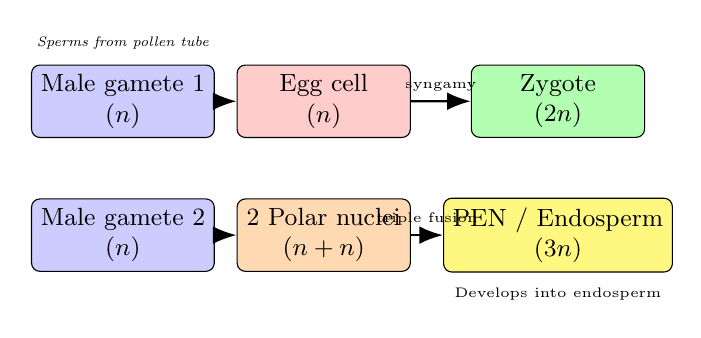
\begin{tikzpicture}[scale=0.85, font=\small,
  box/.style={rectangle, rounded corners=3pt, draw, fill=#1, minimum width=2.2cm, minimum height=0.7cm, align=center},
  arr/.style={-{Latex[length=3mm]}, thick}]
  % Male gametes
  \node[box=blue!20] (mg1) at (-3,2)   {Male gamete 1\\($n$)};
  \node[box=blue!20] (mg2) at (-3,0)   {Male gamete 2\\($n$)};
  % Female structures
  \node[box=red!20]  (egg) at (0,2)    {Egg cell\\($n$)};
  \node[box=orange!30](pn)  at (0,0)   {2 Polar nuclei\\($n + n$)};
  % Products
  \node[box=green!30](zyg) at (3.5,2)  {Zygote\\($2n$)};
  \node[box=yellow!50](pen) at (3.5,0) {PEN / Endosperm\\($3n$)};
  % Arrows
  \draw[arr] (mg1)--(egg);
  \draw[arr] (mg2)--(pn);
  \draw[arr] (egg)--(zyg) node[midway,above]{\tiny syngamy};
  \draw[arr] (pn)--(pen)  node[midway,above]{\tiny triple fusion};
  % Labels
  \node[above=2pt of mg1, font=\tiny\itshape] {Sperms from pollen tube};
  \node[below=2pt of pen, font=\tiny] {Develops into endosperm};
\end{tikzpicture}
\end{center}

Triple fusion: male gamete ($n$) + 2 polar nuclei ($n + n$) $\to$ Primary Endosperm Nucleus ($3n$).\\
This is \textbf{double fertilisation} — unique to angiosperms.
$\boxed{\text{Answer: (B) Endosperm (PEN, }3n\text{)}}$
\end{answerbox}

\begin{notebox}
Double fertilisation = syngamy (egg + sperm $\to$ zygote $2n$) + triple fusion (PEN $3n$).
The endosperm nourishes the developing embryo.
\end{notebox}

\vspace{4pt}

% ── Q2 ───────────────────────────────────────────────────────
\begin{questionbox}{2}{Human Reproduction — Site of Fertilisation}{4}{CO1 / L1}
The site of fertilisation in the female reproductive tract is:

\begin{enumerate}[label=(\Alph*), itemsep=4pt, topsep=6pt]
  \item Uterus
  \item Vagina
  \item Ampullary-isthmic junction of the Fallopian tube
  \item Ovary (follicle)
\end{enumerate}
\end{questionbox}

\begin{answerbox}{C}
\begin{center}
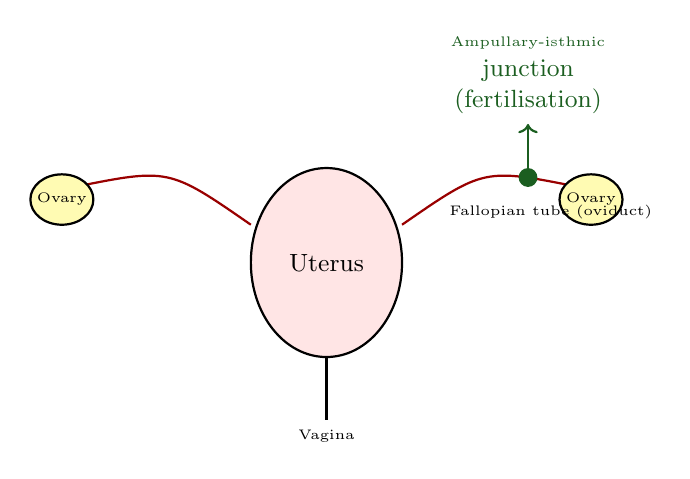
\begin{tikzpicture}[scale=0.8, font=\small]
  % Uterus shape
  \draw[thick,fill=red!10] (0,0) ellipse (1.2 and 1.5);
  \node at (0,0) {Uterus};
  % Fallopian tubes
  \draw[thick,red!60!black] (1.2,0.6) .. controls (2.5,1.5) .. (4,1.2);
  \draw[thick,red!60!black] (-1.2,0.6) .. controls (-2.5,1.5) .. (-4,1.2);
  % Ampulla mark
  \filldraw[accentcolor] (3.2,1.35) circle(4pt);
  \draw[->,thick,accentcolor] (3.2,1.35)--(3.2,2.2) node[above,align=center]{\tiny Ampullary-isthmic\\junction\\(fertilisation)};
  % Ovary
  \draw[thick,fill=yellow!30] (4.2,1.0) ellipse (0.5 and 0.4);
  \node[font=\tiny] at (4.2,1.0) {Ovary};
  \draw[thick,fill=yellow!30] (-4.2,1.0) ellipse (0.5 and 0.4);
  \node[font=\tiny] at (-4.2,1.0) {Ovary};
  % Cervix / vagina
  \draw[thick] (0,-1.5)--(0,-2.5);
  \node[below,font=\tiny] at (0,-2.5) {Vagina};
  % Labels
  \node[font=\tiny,right] at (1.8,0.8) {Fallopian tube (oviduct)};
\end{tikzpicture}
\end{center}
Fertilisation occurs at the \textbf{ampullary-isthmic junction} of the oviduct.
The zygote then undergoes cleavage and travels to the uterus for implantation ($\sim$7 days post-fertilisation).
$\boxed{\text{Answer: (C)}}$
\end{answerbox}

\begin{notebox}
Implantation site: endometrium of uterus.
Fertilisation site: ampullary-isthmic junction.
Sperm capacitation occurs in the female reproductive tract.
\end{notebox}

\vspace{4pt}

% ── Q3 ───────────────────────────────────────────────────────
\begin{questionbox}{3}{Reproductive Health — Contraception}{4}{CO1 / L2}
Which contraceptive method provides protection against \textbf{both} pregnancy
\emph{and} sexually transmitted infections (STIs)?

\begin{enumerate}[label=(\Alph*), itemsep=4pt, topsep=6pt]
  \item Oral contraceptive pills (OCPs)
  \item Intrauterine devices (IUDs)
  \item Condoms (male / female)
  \item Tubectomy (female sterilisation)
\end{enumerate}
\end{questionbox}

\begin{answerbox}{C}
\begin{center}
\renewcommand{\arraystretch}{1.3}
\begin{tabular}{>{\bfseries}p{4cm}>{\centering\arraybackslash}p{2.5cm}>{\centering\arraybackslash}p{2.5cm}}
\toprule
\rowcolor{accentcolor}\color{white}Method & \color{white}Prevents Pregnancy & \color{white}Prevents STI \\
\midrule
\rowcolor{rowB} Oral pills (OCPs) & \checkmark & $\times$ \\
\rowcolor{rowA} IUD & \checkmark & $\times$ \\
\rowcolor{rowB} \textbf{Condoms} & \checkmark & \checkmark \\
\rowcolor{rowA} Tubectomy & \checkmark & $\times$ \\
\bottomrule
\end{tabular}
\end{center}
Condoms are the \emph{only} contraceptive that acts as a physical barrier against both sperm
and pathogens (HIV, HSV, gonorrhoea, etc.). $\boxed{\text{Answer: (C)}}$
\end{answerbox}

\begin{notebox}
\textbf{REMEMBER for NEET:} Condoms = only method that protects against STIs AND pregnancy.
Intrauterine devices (Cu-T, LNG-IUS) — highly effective for pregnancy prevention only.
\end{notebox}

\vspace{4pt}

% ── Q4 ───────────────────────────────────────────────────────
\begin{questionbox}{4}{Molecular Biology — DNA Replication Enzymes}{4}{CO2 / L2}
The enzyme that \textbf{removes RNA primers} and \textbf{fills the gap} with DNA
during replication is:

\begin{enumerate}[label=(\Alph*), itemsep=4pt, topsep=6pt]
  \item DNA Polymerase III
  \item DNA Polymerase I
  \item DNA Ligase
  \item Primase
\end{enumerate}
\end{questionbox}

\begin{answerbox}{B}
\begin{center}
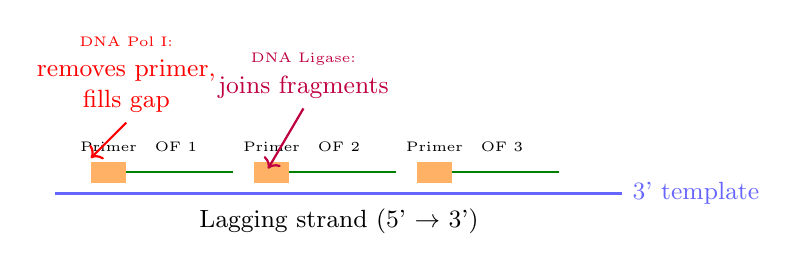
\begin{tikzpicture}[scale=0.9, font=\small,
  arr/.style={-{Latex[length=3mm]}, thick}]
  % Lagging strand
  \draw[thick,blue!60] (0,0)--(8,0) node[right]{\small 3' template};
  % Okazaki fragments
  \foreach \x/\n in {0.5/1, 2.8/2, 5.1/3}{
    \fill[orange!60] (\x,0.15) rectangle (\x+0.5,0.45);
    \draw[thick,green!50!black] (\x+0.5,0.3)--(\x+2,0.3);
    \node[above,font=\tiny] at (\x+0.25,0.45) {Primer};
    \node[above,font=\tiny] at (\x+1.2,0.45) {OF \n};
  }
  % DNA Pol I action
  \draw[->,thick,red] (1.0,1.0)--(0.5,0.5) node[pos=0,above,align=center]{\tiny DNA Pol I:\\removes primer,\\fills gap};
  % DNA Ligase
  \draw[->,thick,purple] (3.5,1.2)--(3.0,0.35) node[pos=0,above,align=center]{\tiny DNA Ligase:\\joins fragments};
  \node[below=2pt] at (4,0) {\small Lagging strand (5' $\to$ 3')};
\end{tikzpicture}
\end{center}

\begin{center}
\renewcommand{\arraystretch}{1.25}
\begin{tabular}{>{\bfseries}p{3.5cm} p{8cm}}
\toprule
\rowcolor{accentcolor}\color{white}Enzyme & \color{white}Function \\
\midrule
\rowcolor{rowB} Helicase & Unwinds and separates DNA strands \\
\rowcolor{rowA} Primase & Synthesises short RNA primers \\
\rowcolor{rowB} DNA Pol III & Main replicating enzyme — extends from primer \\
\rowcolor{rowA} \textbf{DNA Pol I} & \textbf{Removes RNA primer, fills gap with DNA} \\
\rowcolor{rowB} DNA Ligase & Joins Okazaki fragments (seals nicks) \\
\bottomrule
\end{tabular}
\end{center}
$\boxed{\text{Answer: (B) DNA Polymerase I}}$
\end{answerbox}

\begin{notebox}
DNA Pol I has \textbf{dual activity}: 5'$\to$3' exonuclease (removes RNA primer) \emph{and}
5'$\to$3' polymerase (fills the gap with DNA). DNA Ligase then seals the nick.
\end{notebox}

\vspace{4pt}

% ── Q5 ───────────────────────────────────────────────────────
\begin{questionbox}{5}{Evolution — Industrial Melanism}{4}{CO3 / L2}
Industrial melanism in \textit{Biston betularia} (peppered moth) is a classic
example of:

\begin{enumerate}[label=(\Alph*), itemsep=4pt, topsep=6pt]
  \item Natural selection
  \item Genetic drift
  \item Mutation pressure
  \item Founder effect
\end{enumerate}
\end{questionbox}

\begin{answerbox}{A}
\begin{center}
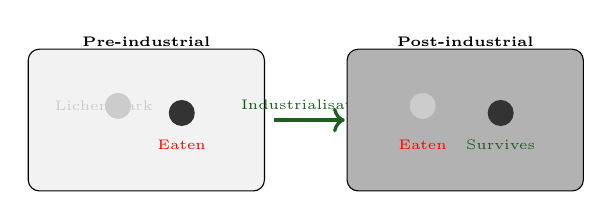
\begin{tikzpicture}[font=\small, scale=0.9]
  % Pre-industrialisation
  \node[draw,rounded corners,fill=gray!10,minimum width=3cm,minimum height=1.8cm] (pre) at (0,0) {};
  \node[above,font=\tiny\bfseries] at (0,0.9) {Pre-industrial};
  \node[font=\tiny,text=white!80!black] at (-0.6,0.2) {Lichen bark};
  \filldraw[white!80!black] (-0.4,0.2) circle (5pt);  % light moth camouflaged
  \filldraw[black!80]        (0.5,0.1)  circle (5pt);  % dark moth visible → eaten
  \node[font=\tiny,red] at (0.5,-0.35) {Eaten};
  % Arrow
  \draw[->,very thick,accentcolor] (1.8,0)--(2.8,0) node[midway,above]{\tiny Industrialisation};
  % Post-industrialisation
  \node[draw,rounded corners,fill=gray!60,minimum width=3cm,minimum height=1.8cm] (post) at (4.5,0) {};
  \node[above,font=\tiny\bfseries] at (4.5,0.9) {Post-industrial};
  \filldraw[white!80!black] (3.9,0.2) circle (5pt);   % light visible → eaten
  \node[font=\tiny,red] at (3.9,-0.35) {Eaten};
  \filldraw[black!80]        (5.0,0.1) circle (5pt);  % dark moth camouflaged
  \node[font=\tiny,accentcolor] at (5.0,-0.35) {Survives};
\end{tikzpicture}
\end{center}

Industrial pollution darkened tree bark; dark (melanic) moths gained a survival advantage
through \textbf{natural selection}. Light moths became more visible to predators.
This is \textbf{directional selection} — allele frequency shifts toward darker phenotype.
$\boxed{\text{Answer: (A) Natural Selection}}$
\end{answerbox}

\begin{notebox}
H.B.D. Kettlewell (1950s) documented this as direct evidence for Darwinian natural selection.
After the Clean Air Act, light moths recovered — showing selection is reversible.
\end{notebox}

\vspace{4pt}

% ── Q6 ───────────────────────────────────────────────────────
\begin{questionbox}{6}{Human Health \& Disease — Malaria Vector}{4}{CO4 / L1}
\textit{Plasmodium falciparum} (malaria parasite) is transmitted by:

\begin{enumerate}[label=(\Alph*), itemsep=4pt, topsep=6pt]
  \item Male \textit{Anopheles} mosquito
  \item Female \textit{Anopheles} mosquito
  \item Female \textit{Culex} mosquito
  \item \textit{Aedes aegypti} mosquito
\end{enumerate}
\end{questionbox}

\begin{answerbox}{B}
\begin{center}
\renewcommand{\arraystretch}{1.3}
\begin{tabular}{>{\bfseries}p{3.5cm} p{3.5cm} p{3.5cm}}
\toprule
\rowcolor{accentcolor}\color{white}Disease & \color{white}Pathogen & \color{white}Vector \\
\midrule
\rowcolor{rowB} \textbf{Malaria}          & \textit{Plasmodium} spp.  & \textbf{Female \textit{Anopheles}} \\
\rowcolor{rowA} Filariasis (elephantiasis) & \textit{Wuchereria}       & Female \textit{Culex} \\
\rowcolor{rowB} Dengue / Chikungunya      & Flavivirus / Alphavirus   & \textit{Aedes aegypti} \\
\rowcolor{rowA} Yellow fever              & Flavivirus                & \textit{Aedes aegypti} \\
\bottomrule
\end{tabular}
\end{center}

The \textbf{female} mosquito requires a blood meal for egg maturation — hence only females transmit
vector-borne diseases. $\boxed{\text{Answer: (B) Female \textit{Anopheles}}}$
\end{answerbox}

\begin{notebox}
Malaria life cycle key stages:
\textbf{Liver} (exo-erythrocytic) $\to$ \textbf{RBC} (erythrocytic, fever stage) $\to$
\textbf{Mosquito} (sexual stage, sporogony).
\end{notebox}

\vspace{4pt}

% ── Q7 ───────────────────────────────────────────────────────
\begin{questionbox}{7}{Food Production — Somatic Hybridisation}{4}{CO4 / L2}
Somatic hybridisation involves:

\begin{enumerate}[label=(\Alph*), itemsep=4pt, topsep=6pt]
  \item Fusion of two gametes from different plant species
  \item Fusion of protoplasts from two different plant species
  \item Crossing two inbred lines to produce a hybrid
  \item Insertion of a foreign gene into a plant genome
\end{enumerate}
\end{questionbox}

\begin{answerbox}{B}
\begin{center}
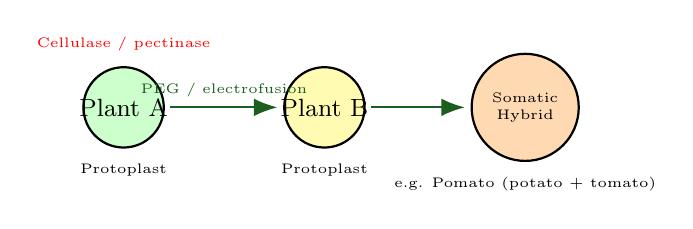
\begin{tikzpicture}[font=\small, scale=0.85,
  arr/.style={-{Latex[length=3mm]}, thick, accentcolor}]
  % Plant A protoplast
  \draw[thick,fill=green!20] (-3,0) circle (0.6) node{Plant A};
  \node[below,font=\tiny] at (-3,-0.7) {Protoplast};
  % Plant B protoplast
  \draw[thick,fill=yellow!30] (0,0) circle (0.6) node{Plant B};
  \node[below,font=\tiny] at (0,-0.7) {Protoplast};
  % Fusion arrow
  \draw[arr] (-2.3,0)--(-0.7,0) node[midway,above]{\tiny PEG / electrofusion};
  % Somatic hybrid
  \draw[thick,fill=orange!30] (3,0) circle (0.8);
  \node[align=center,font=\tiny] at (3,0) {Somatic\\Hybrid};
  \draw[arr] (0.7,0)--(2.1,0);
  \node[below,font=\tiny] at (3,-0.9) {e.g. Pomato (potato + tomato)};
  % Cell wall removal
  \node[above,font=\tiny,red] at (-3,0.7) {Cellulase / pectinase};
\end{tikzpicture}
\end{center}

Somatic hybridisation = fusion of \textbf{protoplasts} (cells with cell walls removed by cellulase/pectinase)
from two different plant species, bypassing sexual incompatibility barriers.
$\boxed{\text{Answer: (B)}}$
\end{answerbox}

\begin{notebox}
Famous example: \textbf{Pomato} = potato (\textit{Solanum tuberosum}) + tomato (\textit{Solanum lycopersicum}).
The hybrid was created but proved commercially non-viable (poor tubers AND poor fruits).
\end{notebox}

\vspace{4pt}

% ── Q8 ───────────────────────────────────────────────────────
\begin{questionbox}{8}{Microbes in Human Welfare — Yeast}{4}{CO4 / L1}
\textit{Saccharomyces cerevisiae} is used industrially in the production of:

\begin{enumerate}[label=(\Alph*), itemsep=4pt, topsep=6pt]
  \item Penicillin (antibiotic)
  \item Biogas (methane)
  \item Ethanol and for leavening bread
  \item Curd / yoghurt
\end{enumerate}
\end{questionbox}

\begin{answerbox}{C}
\begin{center}
\renewcommand{\arraystretch}{1.3}
\begin{tabular}{>{\bfseries}p{4cm} p{3cm} p{4cm}}
\toprule
\rowcolor{accentcolor}\color{white}Microbe & \color{white}Product & \color{white}Use \\
\midrule
\rowcolor{rowB} \textbf{\textit{S. cerevisiae}} & \textbf{Ethanol, CO$_2$} & \textbf{Brewing, baking} \\
\rowcolor{rowA} \textit{Penicillium notatum}  & Penicillin     & Antibiotic \\
\rowcolor{rowB} \textit{Methanobacterium}     & Methane        & Biogas \\
\rowcolor{rowA} \textit{Lactobacillus}        & Lactic acid    & Curd / yoghurt \\
\rowcolor{rowB} \textit{Aspergillus niger}    & Citric acid    & Food industry \\
\bottomrule
\end{tabular}
\end{center}
Fermentation: $\text{C}_6\text{H}_{12}\text{O}_6 \longrightarrow 2\,\text{C}_2\text{H}_5\text{OH} + 2\,\text{CO}_2$
\quad (anaerobic).\quad CO$_2$ causes bread to rise. $\boxed{\text{Answer: (C)}}$
\end{answerbox}

\begin{notebox}
\textit{S. cerevisiae} = baker's yeast AND brewer's yeast. It is also used to produce
insulin (recombinant), hepatitis B vaccine, and as a model organism in cell biology.
\end{notebox}

\vspace{4pt}

% ── Q9 ───────────────────────────────────────────────────────
\begin{questionbox}{9}{Biotechnology — Restriction Enzymes}{4}{CO5 / L2}
Restriction enzymes cut DNA at specific sequences called:

\begin{enumerate}[label=(\Alph*), itemsep=4pt, topsep=6pt]
  \item Promoter sequences
  \item Palindromic recognition sequences
  \item Satellite (repetitive) sequences
  \item Telomeric sequences
\end{enumerate}
\end{questionbox}

\begin{answerbox}{B}
A \textbf{palindromic sequence} reads the same on both strands in the 5'$\to$3' direction:

\begin{center}
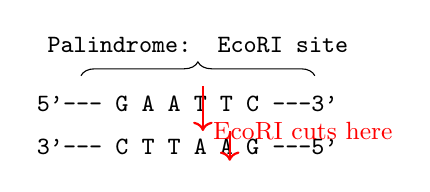
\begin{tikzpicture}[font=\small\ttfamily, scale=0.9]
  % Top strand
  \node at (0,0.6) {5'--- G A A T T C ---3'};
  % Bottom strand
  \node at (0,0)   {3'--- C T T A A G ---5'};
  % Cut arrows
  \draw[->,thick,red] (0.22,0.85)--(0.22,0.22) node[right,font=\small\rmfamily]{\small EcoRI cuts here};
  \draw[->,thick,red] (0.6,0.22)--(0.6,-0.2);
  % Braces
  \draw[decorate,decoration={brace,amplitude=5pt}] (-1.5,1.0)--(1.8,1.0) node[midway,above=5pt]{\small Palindrome: EcoRI site};
\end{tikzpicture}
\end{center}

EcoRI recognition site: 5'-\texttt{GAATTC}-3' / 3'-\texttt{CTTAAG}-5'.
Cuts between G and A on both strands $\to$ produces \textbf{sticky ends}.
$\boxed{\text{Answer: (B) Palindromic recognition sequences}}$
\end{answerbox}

\begin{notebox}
Types of ends after restriction digestion:
\textbf{Sticky ends} (staggered cuts, e.g. EcoRI, BamHI) — preferred for cloning.
\textbf{Blunt ends} (straight cuts, e.g. SmaI) — harder to ligate efficiently.
\end{notebox}

\vspace{4pt}

% ── Q10 ──────────────────────────────────────────────────────
\begin{questionbox}{10}{Ecosystem — Energy Pyramid}{4}{CO5 / L2}
The pyramid of energy in an ecosystem is \textbf{always}:

\begin{enumerate}[label=(\Alph*), itemsep=4pt, topsep=6pt]
  \item Inverted
  \item Upright (erect)
  \item Spindle-shaped
  \item Can be inverted in aquatic ecosystems
\end{enumerate}
\end{questionbox}

\begin{answerbox}{B}
\begin{center}
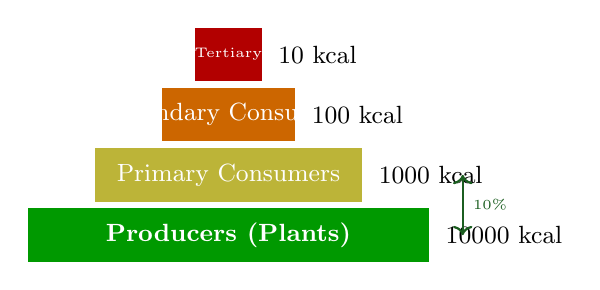
\begin{tikzpicture}[scale=0.85, font=\small]
  % Energy pyramid
  \fill[green!60!black]  (-3,0)    rectangle (3,0.8);
  \fill[yellow!70!black] (-2,0.9)  rectangle (2,1.7);
  \fill[orange!80!black] (-1,1.8)  rectangle (1,2.6);
  \fill[red!70!black]    (-0.5,2.7) rectangle (0.5,3.5);
  % Labels
  \node[white,font=\bfseries\small] at (0,0.4)  {Producers (Plants)};
  \node[white,font=\small]          at (0,1.3)  {Primary Consumers};
  \node[white,font=\small]          at (0,2.2)  {Secondary Consumers};
  \node[white,font=\tiny]           at (0,3.1)  {Tertiary};
  % Energy values
  \node[right] at (3.1,0.4)  {\small $10000$ kcal};
  \node[right] at (2.1,1.3)  {\small $1000$ kcal};
  \node[right] at (1.1,2.2)  {\small $100$ kcal};
  \node[right] at (0.6,3.1)  {\small $10$ kcal};
  % 10% law label
  \draw[<->,thick,accentcolor] (3.5,0.4)--(3.5,1.3) node[midway,right]{\tiny 10\%};
\end{tikzpicture}
\end{center}

Only $\sim$10\% of energy is transferred to the next trophic level (Lindemann's 10\% law).
The pyramid of energy is \textbf{always upright} — energy always decreases up the trophic levels.
Unlike biomass or numbers pyramids, the \emph{energy pyramid can never be inverted}.

$\boxed{\text{Answer: (B) Always upright}}$
\end{answerbox}

\begin{notebox}
\textbf{Pyramid comparison (NEET):}
Numbers pyramid — can be inverted (e.g. one tree, many insects).
Biomass pyramid — can be inverted (aquatic: phytoplankton $<$ zooplankton biomass at a moment).
Energy pyramid — \textbf{ALWAYS upright, no exception}.
\end{notebox}

\label{LastPage}
\end{document}
